% ============================================================================
%  B.Tech Project (BTP) -- Mid-semester report
%
%  BEFORE SUBMITTING, FILL IN the three commands marked FILL THESE IN below:
%    \supervisor, \rollno, \dept
%
%  OVERLEAF SETUP
%    1. New Project -> Blank Project, paste this file as main.tex
%    2. Upload the five PDFs from evaluation/results/figures/ into a folder
%       called figures/
%    3. Compile with pdfLaTeX
%
%  FRAMING NOTE (for me, not the examiner):
%  The project is an AGENT for time-series modelling across domains. Anomaly
%  detection is the FIRST capability delivered and validated, not the project
%  itself. Section 1 states the whole goal, Table 1 shows the full task/domain
%  matrix with status, and the end-semester report continues the same table.
% ============================================================================
\documentclass[11pt,a4paper]{article}

\usepackage[margin=2.0cm]{geometry}
\usepackage{graphicx}
\usepackage{booktabs}
\usepackage{caption}
\usepackage[hidelinks]{hyperref}
\usepackage{microtype}
\usepackage{titlesec}
\usepackage{enumitem}
\usepackage{array}

\captionsetup{font=small,labelfont=bf,skip=4pt}
\titleformat{\section}{\normalfont\large\bfseries}{\thesection.}{0.6em}{}
\titlespacing*{\section}{0pt}{9pt}{4pt}
\titleformat{\subsection}{\normalfont\normalsize\bfseries}{\thesubsection}{0.6em}{}
\titlespacing*{\subsection}{0pt}{6pt}{3pt}
\setlist{nosep,leftmargin=1.3em}
\setlength{\parskip}{3pt}
\newcommand{\done}{\textbf{done}}
\newcommand{\next}{planned}

% ---------------------------- FILL THESE IN -------------------------------
\newcommand{\supervisor}{[Supervisor name], [Department]}
\newcommand{\rollno}{EP230051010}
\newcommand{\dept}{Department of Electrical Engineering}
% --------------------------------------------------------------------------

\begin{document}

% ========================= TITLE BLOCK ====================================
\begin{center}
  {\large B.Tech Project \textbar{} Mid-Semester Report}\\[0.6em]
  \rule{\textwidth}{0.8pt}\\[0.7em]
  {\LARGE\bfseries A Multi-Agent System for Time-Series\\[0.25em]
   Modelling across Scientific and Financial Domains}\\[0.5em]
  {\large Mid-semester deliverable: the agent framework, and its first
   capability validated end to end}\\[0.6em]
  \rule{\textwidth}{0.8pt}\\[1.0em]

  \begin{tabular}{r@{\hspace{0.9em}}l}
    \textbf{Submitted by}  & Kaveri Neeli (\rollno) \\
    \textbf{Supervisor}    & \supervisor \\
    \textbf{Department}    & \dept \\
    \textbf{Institute}     & Indian Institute of Technology Indore \\
    \textbf{Date}          & September 2026 \\
  \end{tabular}
\end{center}
\vspace{0.4em}

% ========================= ABSTRACT =======================================
\noindent\rule{\textwidth}{0.4pt}\\[0.2em]
\begin{center}\textbf{Abstract}\end{center}
\vspace{-0.5em}
{\small\noindent
The goal of this project is an agent that performs time-series modelling across
unrelated domains, choosing the right analysis for a question instead of
running a fixed pipeline. This semester I built the framework and validated it
on the first of its tasks. The framework is a registry of 20 models spanning 10
task types and 4 domains, with a capability filter that selects among them.
Across 123 labelled queries that filter routes correctly 95.9\% of the time
against 83.7\% for a language model, in under a second where the model needs 41
minutes. I then used the framework to take one task, anomaly detection, all the
way through on two domains: 440 Kepler light curves labelled from NASA
ephemerides, and seven years of Indian equity returns labelled from a calendar
fixed in advance. Under held-out evaluation all 22 detectors land within 0.04
PR-AUC of a rule that learns nothing, and the gap between in-sample and
held-out scores tracks model capacity rather than skill, from $1.0\times$ to
$6.4\times$. The limiting factor is the representation, which I show by
changing the question: a Box Least Squares period search recovers 61\% of
orbital periods across all 440 targets.\par}
\vspace{0.2em}
\noindent\rule{\textwidth}{0.4pt}

% ========================= 1. INTRODUCTION ================================
\section{Project Goal and Objectives}

Time-series questions come in several kinds. \emph{What will this be worth next
month?} is forecasting. \emph{Which days were unusual?} is anomaly detection.
\emph{How likely is an event in the next 24 hours?} is a point-process problem.
\emph{How much could I lose?} is risk. Each needs a different model, and the
right model also depends on the domain the data came from.

Most systems handle this with a fixed pipeline per domain. The goal of this
project is different: \textbf{one agent that decides, for any question, which
analysis to run, and chooses on measured evidence rather than a language
model's judgement.} Table~\ref{tab:matrix} shows the space the agent covers and
what has been completed so far.

\begin{table}[h]
\centering\small
\caption{Task and domain coverage. This report delivers the framework (all
columns) and takes anomaly detection through full validation on two domains.}
\label{tab:matrix}
\begin{tabular}{@{}lcccl@{}}
\toprule
\textbf{Task} & \textbf{Astronomy} & \textbf{Finance} & \textbf{Solar} &
\textbf{Status at mid-semester} \\
\midrule
Anomaly detection      & 3 & 2 & -- & \done: 22 detectors, held-out, both domains \\
Model selection        & \multicolumn{3}{c}{framework-wide} & \done: 95.9\% on 123 queries \\
Structure profiling    & \multicolumn{3}{c}{framework-wide} & \done: 10/10 on unseen series \\
Forecasting a value    & -- & 3 & -- & built, not yet validated to this standard \\
Event probability      & -- & 1 & 3 & built, not yet validated \\
Risk assessment        & -- & 1 & -- & built, validation in progress \\
Sentiment, lookups     & 1 & 2 & -- & supporting tasks \\
\bottomrule
\end{tabular}
\end{table}

\subsection*{Objectives}
\begin{enumerate}[label=\textbf{O\arabic*.}]
  \item Build an agent that routes a natural-language question to the correct
        analysis, with no language model in the decision path.
  \item Make model selection evidence-based, so every model in the registry
        carries a skill figure measured out of sample.
  \item Validate the framework by taking one task end to end across two
        unrelated domains, to a standard where the result can be trusted.
  \item From that validation, identify what actually limits performance, and
        demonstrate a method that overcomes it.
\end{enumerate}

\subsection*{Why anomaly detection was chosen as the first task}
It is the hardest of the four to evaluate honestly, so it exercises the
framework's weakest point. It also exists in both astronomy and finance in
structurally opposite forms: a planetary transit is a shallow dip that
\emph{repeats} every few days, while a market crash is a large move that
happens \emph{once}. If the selection layer can handle a task whose correct
model inverts between domains, the design generalises. Solar-flare forecasting,
the risk layer and cross-sectional equity work are running and appear in the
plan in Section~7.

% ========================= 2. LITERATURE ==================================
\section{Literature Review}

\textbf{Benchmarks in this field are unreliable.} Wu and Keogh~\cite{wu2021}
examined the Yahoo, Numenta, NASA and OMNI archives and found most problems
suffer from at least one of four flaws: triviality, unrealistic anomaly
density, mislabelled ground truth, and run-to-failure bias. Roughly 90\% yield
to a single line of arithmetic, and their conclusion is that on such data no
level of reported performance implies a method is useful.

\textbf{The scoring protocol is also compromised.} Kim et al.~\cite{kim2022}
showed that \emph{point adjustment}, the dominant convention, lets a random
anomaly score reach state-of-the-art $F_1$, because marking a whole segment
correct for one lucky hit rewards noise.

\textbf{Complex models do not reliably win.} A 2024 benchmark of 1{,}070 series
across 40 datasets~\cite{tsbad2024} concluded that simpler architectures and
statistical methods often outperform neural ones. Work at ICLR 2026 found five
foundation model families failing to beat moving-window variance, and gave the
reason: anomalies are not consistently harder to reconstruct or forecast.

\textbf{For transit detection}, Box Least Squares~\cite{kovacs2002} remains
standard, and the matrix profile~\cite{yeh2016} is the canonical tool for
subsequence anomalies. I use both, and the contrast between them is informative.

\textbf{Gap addressed here.} These critiques are widely cited but rarely
applied by authors to their own data. I run the four-flaw audit on my own
datasets before reporting any result, and report in-sample and held-out scores
side by side so the difference is visible. That discipline is what lets the
registry's skill figures be trusted, which is what the selection layer depends
on.

% ========================= 3. METHODOLOGY =================================
\section{System Design and Methodology}

\subsection{Agent architecture}
Figure~\ref{fig:pipeline} shows the query pipeline. A question is parsed into a
\emph{domain} and a \emph{task}. The registry is filtered to models that can
actually run given the available inputs. One is selected on recorded skill, it
executes, and a rule-based explanation is composed from the same features the
model used. Only the final phrasing step calls a language model.

\begin{figure}[t]
  \centering
  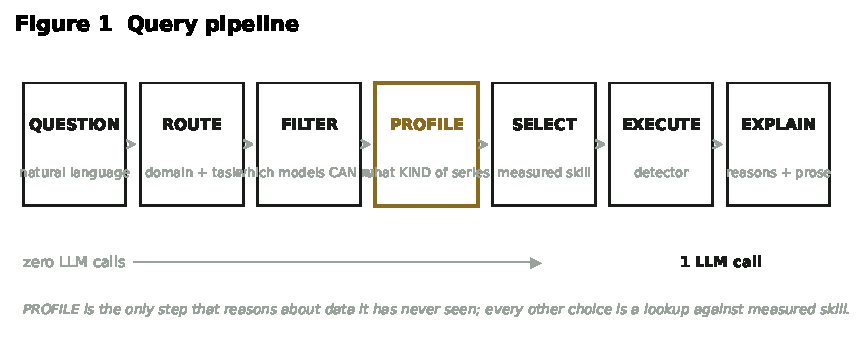
\includegraphics[width=0.92\linewidth]{figures/fig_pipeline.pdf}
  \caption{Query pipeline. Every decision except the final phrasing is made in
  Python. Profiling is the only step that reasons about unseen data.}
  \label{fig:pipeline}
\end{figure}

Each registry entry declares its domain, task, required inputs, return type and
measured skill. Separating domain (which data) from task (which model) keeps
routing out of the control flow, so adding a model is one registry entry rather
than an edit to a branch. That is what makes the design extensible to the tasks
still to come in Table~\ref{tab:matrix}.

\subsection{Structure profiling}
Before selecting a model the agent inspects the series itself, using the ratio
of the Lomb--Scargle periodogram peak to its background. Across ten Kepler
targets and ten equities the two populations had medians of 1{,}939 and 12.4
with no overlap, and a single threshold classified all twenty correctly.

This decision inverts which detector is correct. Scored as a \emph{discord} (a
subsequence unlike any other) the matrix profile reaches ROC 0.303 on
KIC~10074466, below chance. Scored as a \emph{motif} it reaches 0.697. A
transit recurs 221 times, making it the \emph{least} unusual feature of its own
light curve, so generic anomaly detection hunts the opposite of what is there.

\subsection{Datasets and labelling}
\textbf{Astronomy.} 440 Kepler light curves (217 confirmed planets, 223 false
positives), windowed at 12~hours with a 3~hour stride, giving 384{,}281 windows
at 24.4\% positive. A window is a transit if it overlaps $T_0 + nP$ from NASA's
ephemeris. That is orbital mechanics, and it never touches the brightness being
scored.

\textbf{Finance.} An equal-weighted index of the 50 most liquid NSE names,
2019--2026, windowed at 21 trading days, giving 1{,}891 windows at 2.2\%
positive, labelled from a pre-registered calendar of budget sessions, election
results and ten documented shocks.

\textbf{Circularity, and a mistake I made.} An earlier version labelled
astronomy windows by thresholding their own \emph{depth}, then evaluated
detectors that look for deep dips. That is grading an exam with the student's
own answer sheet. When I caught it, the measured inflation was $+0.11$~AUC.
Solar flares are excluded from this task for the strongest version of the same
problem: a flare's class is \emph{defined} by an X-ray threshold, so detecting
flares from X-ray flux cannot fail.

\subsection{Evaluation protocol}
PR-AUC is the decision metric because it is floored at the base rate and stays
interpretable when anomalies are rare, with ROC-AUC beside it. I do not apply
point adjustment, for the reason in Section~2. Every model ran once, at a
configuration fixed before I saw any result. Splits are temporal for equity and
by-target for Kepler, stratified by per-target prevalence after my first
attempt produced halves at 17.9\% and 42.8\% positive.

% ========================= 4. IMPLEMENTATION ==============================
\section{Implementation}

The system is Python, organised so the domain-neutral components cannot see
domain-specific information. The \texttt{anomaly} package holds the scoring
contract and windowing, 22 detectors across six families, the label sources,
the four-flaw audit, held-out splitting with prevalence stratification, the
Lomb--Scargle profiler and a parallelised grid runner.
\texttt{astronomy/transit\_search} implements the period search, and
\texttt{agents/model\_registry} holds the 20 models of
Table~\ref{tab:matrix} with their declared capabilities and skill.

Detectors span thresholds (z-score, Hampel/MAD), density (isolation forest,
Mahalanobis, local outlier factor, one-class SVM, elliptic envelope),
reconstruction (PCA and LSTM autoencoders, spectral PCA, latent isolation
forest), latent-state (hidden Markov model, GARCH residuals) and four matrix
profile configurations, plus two deliberate no-skill floors and a supervised
ceiling. Results are served through a Streamlit dashboard and a chatbot, with
all 440 astronomy targets precomputed into MongoDB for 4.5~ms lookups.

% ========================= 5. RESULTS =====================================
\section{Results and Discussion}

\subsection{Model selection (O1, O2)}
On 123 labelled queries covering canonical phrasings, paraphrases, adversarial
cases and questions no model can answer, the capability filter reached 95.9\%,
the language model alone 83.7\%, and the two combined 95.1\%
(Figure~\ref{fig:routing}). The filter is not merely cheaper. It is more
accurate, and adding the language model costs accuracy as well as time.

\begin{figure}[t]
  \centering
  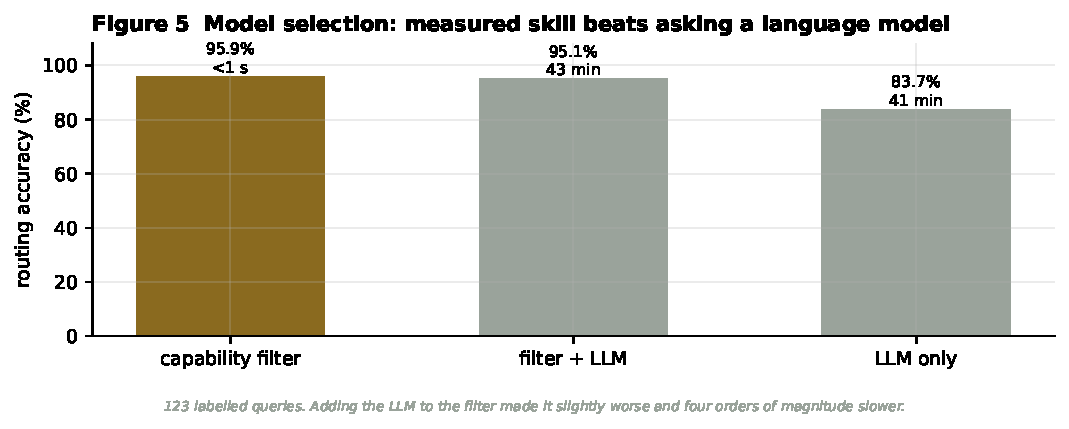
\includegraphics[width=0.56\linewidth]{figures/fig_routing.pdf}
  \caption{Model selection on 123 labelled queries.}
  \label{fig:routing}
\end{figure}

\subsection{Dataset audit}
Equity passes all four flaw checks. Kepler passes three and warns on anomaly
density at 24.4\% positive, genuine because short-period planets transit almost
continuously, but above what the literature treats as realistic.

\subsection{Detector comparison (O3)}
Figure~\ref{fig:grid} and Table~\ref{tab:results} give the held-out results. On
Kepler the best detector beats the strongest no-skill floor by 0.0102~PR-AUC,
$1.12\times$ chance against the floor's $1.08\times$. The supervised ceiling, a
gradient-boosted model trained directly on the labels, reaches only 0.2555 and
is outscored by three unsupervised detectors. On equity the margin is 0.0030.

\begin{figure}[t]
  \centering
  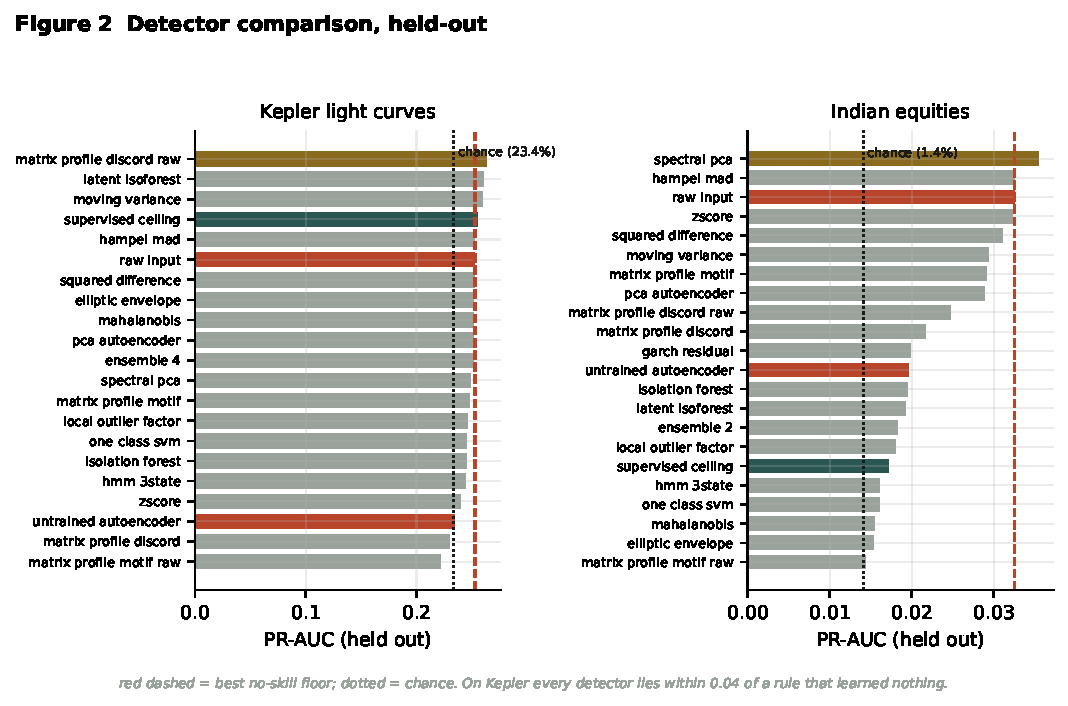
\includegraphics[width=0.88\linewidth]{figures/fig_grid.pdf}
  \caption{Twenty-two detectors across five families, scored on held-out data.}
  \label{fig:grid}
\end{figure}

\begin{table}[h]
\centering\small
\caption{Held-out PR-AUC for selected detectors. Lift is PR-AUC divided by the
base rate; inflation is in-sample PR-AUC divided by held-out.}
\label{tab:results}
\begin{tabular}{@{}llrrr@{}}
\toprule
Domain & Detector & PR-AUC & Lift & Inflation \\
\midrule
Kepler & matrix profile (discord, raw) & 0.2630 & 1.12$\times$ & 1.1$\times$ \\
Kepler & latent isolation forest       & 0.2605 & 1.11$\times$ & 1.2$\times$ \\
Kepler & \emph{supervised ceiling}     & 0.2555 & 1.09$\times$ & 1.3$\times$ \\
Kepler & \emph{raw input} (floor)      & 0.2528 & 1.08$\times$ & 1.2$\times$ \\
\midrule
Equity & spectral PCA (FFT + PCA)      & 0.0355 & 2.52$\times$ & 1.5$\times$ \\
Equity & \emph{raw input} (floor)      & 0.0325 & 2.31$\times$ & 2.0$\times$ \\
Equity & LSTM autoencoder              & 0.0270 & 1.92$\times$ & --- \\
Equity & one-class SVM                 & 0.0161 & 1.14$\times$ & 6.4$\times$ \\
\bottomrule
\end{tabular}
\end{table}

\subsection{In-sample scores overstate performance in proportion to capacity}
The ratio of in-sample to held-out PR-AUC climbs steadily with how much a model
can memorise: $1.0$--$1.1\times$ for the parameter-free matrix profile,
$2.0\times$ for threshold rules, $2.9\times$ for isolation forest, $4.7\times$
for local outlier factor and $6.4\times$ for a one-class SVM
(Figure~\ref{fig:inflation}). Evaluated transductively, the ordinary convention
in unsupervised anomaly detection, the one-class SVM looks like the best equity
detector at $4.62\times$ lift. Held out it manages $1.14\times$. I had already
recorded it as the winner before the held-out split existed. This is also why
the registry stores held-out figures: a selection layer fed transductive scores
would have picked that model.

\begin{figure}[t]
  \centering
  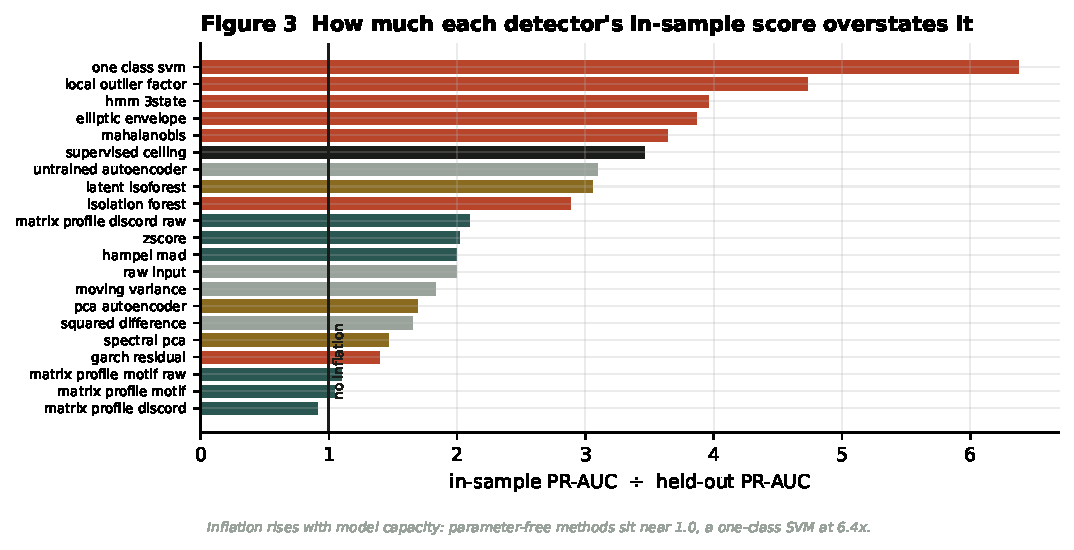
\includegraphics[width=0.70\linewidth]{figures/fig_inflation.pdf}
  \caption{In-sample scores overstate held-out performance in proportion to
  model capacity.}
  \label{fig:inflation}
\end{figure}

\subsection{The representation is the limiting factor (O4)}
On Kepler, 44.2\% of labelled transits are no more extreme than a typical
non-transit window at this resolution, and the supervised ceiling reaches only
$1.09\times$ chance. The window statistics do not contain the signal, so no
detector working on them can find it. An LSTM autoencoder, added to test
whether temporal order inside a window helps, reached $1.92\times$ on equity
against a threshold rule's $2.31\times$, at roughly $250\times$ the compute.

Changing the question rather than the algorithm resolves it. Box Least Squares
folds the light curve on thousands of candidate periods and stacks every
repetition (Figure~\ref{fig:transit}). Across all 440 targets it produces a
significant periodogram peak for 91.4\% and recovers the published period to
within 1\% for 60.9\%, at median significance 42.3 and median period error
0.005\%. The gap between those figures is harmonic locking: 33.6\% of targets
return $P/2$, $P/3$ or $2P$, so the signal is present and only the fold
multiple is wrong.

\begin{figure}[t]
  \centering
  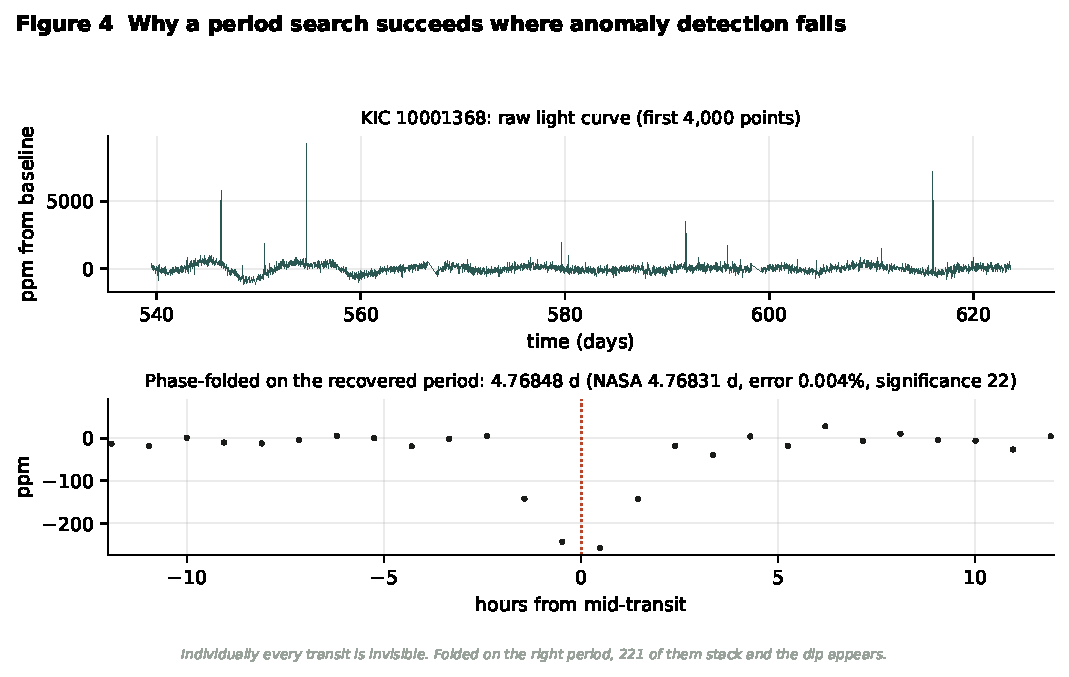
\includegraphics[width=0.70\linewidth]{figures/fig_transit.pdf}
  \caption{A single transit is invisible in the raw series. Folded on the
  recovered period, 221 of them stack into a clear 250~ppm dip.}
  \label{fig:transit}
\end{figure}

\subsection{Configuration inverts between domains}
The same algorithm needs opposite settings in the two domains. On Kepler the
matrix profile must be read as a motif under $z$-normalised distance, because
transits repeat and their depth varies by star. On equity it must be read as a
discord under un-normalised distance, because shocks are unique and the size of
the move is the signal. Getting both axes wrong scores $0.95\times$, below
chance. This is the clearest justification for the profiling step, and the
reason the same task needed different models in the two domains.

% ========================= 6. CONCLUSION ==================================
\section{Conclusion}

Against the objectives: the agent routes at 95.9\% with no language model in
the decision path (O1); every registry entry now carries an out-of-sample skill
figure, and the inflation result shows why that had to be out-of-sample (O2);
anomaly detection was taken end to end on two unrelated domains under held-out
evaluation (O3); and the limiting factor was identified as representational and
overcome with a period search recovering 61\% of orbital periods (O4).

The framework is therefore validated on its first task, and the finding from
that task is negative and reported as such: 22 detectors across two domains all
sit within 0.04 PR-AUC of a rule that learns nothing, and whatever advantage
they appear to hold in-sample scales with capacity rather than skill.

% ========================= 7. PLAN ========================================
\section{Work Plan for the Second Half}

The second half fills in the remaining rows of Table~\ref{tab:matrix}, taking
each to the same evidential standard as anomaly detection.

\begin{table}[h]
\centering\small
\begin{tabular}{@{}llp{7.6cm}@{}}
\toprule
\textbf{Weeks} & \textbf{Task added} & \textbf{Detail} \\
\midrule
1--2  & Risk assessment   & Markov regime model and regime-conditional
                            Value-at-Risk, which passes Kupiec and
                            Christoffersen coverage tests that the
                            unconditional version fails \\
3--4  & Third domain      & Blazar light curves from the Fermi-LAT repository.
                            The profiler predicts these behave like equities
                            rather than Kepler, which is a testable prediction \\
5--6  & Forecasting       & Bring the forecasting and event-probability models
                            to the same held-out standard, and register their
                            skill \\
7--8  & Ablation          & Bare language model vs.\ retrieval vs.\ full agent,
                            isolating what the architecture contributes \\
9--10 & Final report      & Writing and defence preparation \\
\bottomrule
\end{tabular}
\end{table}

% ========================= REFERENCES =====================================
\begin{thebibliography}{9}\small
\bibitem{wu2021} R.~Wu and E.~J.~Keogh. Current time series anomaly detection
benchmarks are flawed and are creating the illusion of progress.
\emph{IEEE Transactions on Knowledge and Data Engineering}, 2022.
\bibitem{kim2022} S.~Kim, K.~Choi, H.-S.~Choi, B.~Lee and S.~Yoon. Towards a
rigorous evaluation of time-series anomaly detection. \emph{AAAI}, 2022.
\bibitem{tsbad2024} Q.~Liu and J.~Paparrizos. The elephant in the room: towards
a reliable time-series anomaly detection benchmark. \emph{NeurIPS Datasets and
Benchmarks Track}, 2024.
\bibitem{kovacs2002} G.~Kov\'acs, S.~Zucker and T.~Mazeh. A box-fitting
algorithm in the search for periodic transits. \emph{Astronomy \&
Astrophysics}, 391:369--377, 2002.
\bibitem{yeh2016} C.-C.~M.~Yeh et al. Matrix profile I: all pairs similarity
joins for time series. \emph{IEEE ICDM}, 2016.
\end{thebibliography}

\end{document}
